\chapter{Results}
De sidste tests som vi har udført og dermed de sidste målinger / resultater. Det målesæt vi bruger bør være det sæt der gav tendenslinjen 254x+0












\chapter{Improvements}
This chapter contains thoughs about the improvements we want to make to our system but did not have the time to do.
\section{Using the system as an actual musical instrument}
\subsection{Playing notes}
The system outputs a sine wave sound. This is great for demonstrative purposes but might not be as pleasant to listen to. What makes a musical sound or "note" pleasant to listen to is harmonics. Most musical tones are composed of fundamental tone and multiple overtones. A sequence of a fundamental tone and 3 overtones would then consist of 4 harmonics. Mathematically, tones are composed of the fundamental frequency and multiples of fundamental frequency like so:\\
\begin{itemize}
\item 1 * freq : fundamental tone : 1st harmonic
\item 2 * freq : 1st overtone     : 2nd harmonic
\item 3 * freq : 2nd overtone     : 3rd harmonic
\item n * freq : (n-1) overtone   : nth harmonic
\end{itemize}
This is also shows on figure ~\ref{fig:harmonics}. To produce such a signal on an embedded unit we would have to use the principle of Fourier series and add the different frequency components together. 
\begin{figure}[hbpt]
\centering
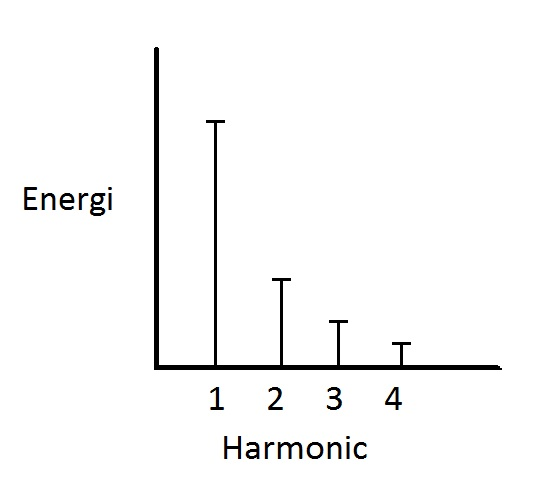
\includegraphics[scale=0.5]{billeder/harmonics}
\caption{n = 4 : harmonics}
\label{fig:harmonics}
\end{figure}
\subsection{Select distance intervals equal to notes}
The idea would be to set intervals for distance much like the distance between keys on a piano. This is shown on figure~\ref{fig:pianokeys}. The idea would then be that you would place a person or an item in the interval and then play a tone with a fixed rate. The rates would then be configurable with buttons on the blackfin for instance.
\begin{figure}[hbpt]
\centering
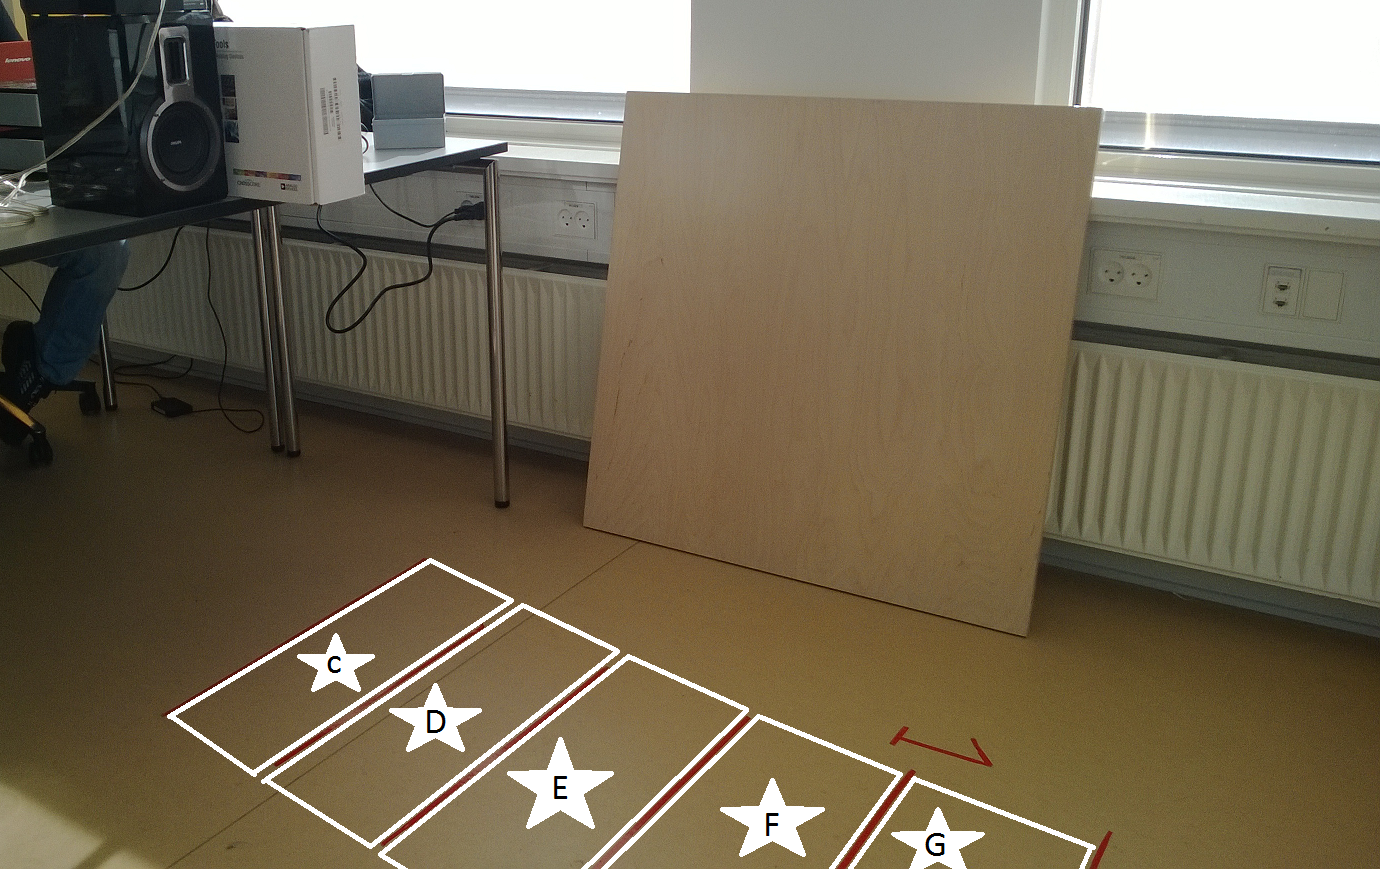
\includegraphics[scale=0.3]{billeder/pianokeyground}
\caption{Piano Keys drawn in front of the system}
\label{fig:pianokeys}
\end{figure}